\documentclass[../book_jiriki_calc]{subfiles}

\begin{document}

\section{グラフを描いて2変数関数を見る}

2変数関数$f(x, y)$が与えられたとき、変数$x,\,y$を自由に動かして点$(x, y, f(x,y))$を$xyz$空間でプロットして得られる曲面を\keyword{$z= f(x, y)$のグラフ}という。

\br

$f(x,y)$が地点$(x, y)$の標高の場合は、この$z=f(x,y)$のグラフが表す曲面はこの野山の地表にほかならない。
\begin{itemize}
  \item 2変数関数$f(x, y)$をグラフで可視化すると、野山の形状になる
  \item 野山の形状から標高を考えると、2変数関数$f(x, y)$になる
\end{itemize}

\sectionline

\subparagraph{$f(x,y)=x^2+y^2$のグラフ}\quad

このグラフは、壺のような形になっている

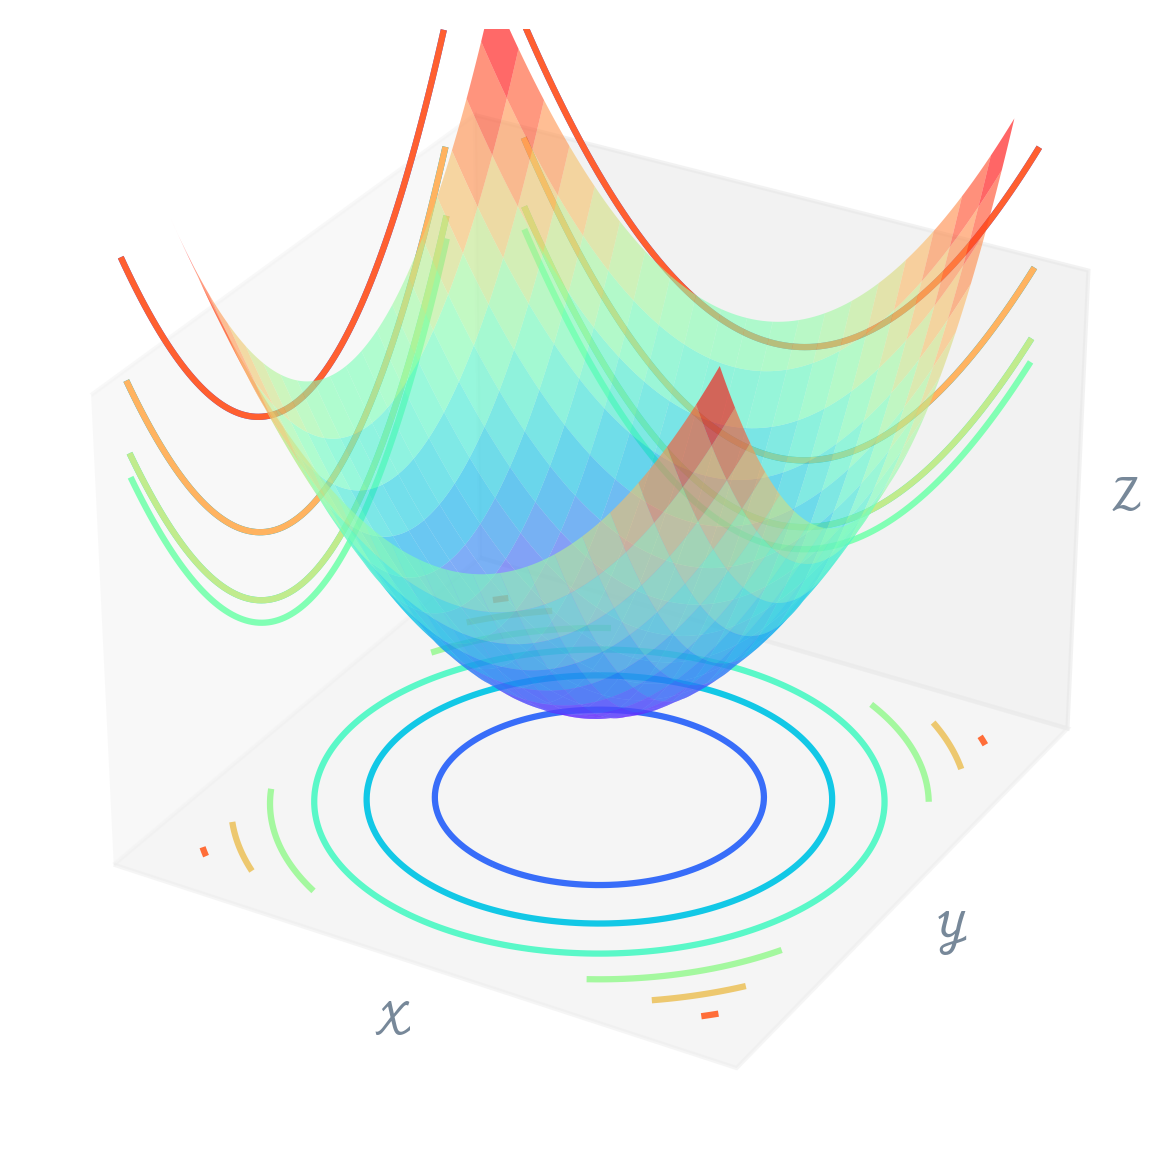
\includegraphics[width=0.9\linewidth]{./python/graph_x-pow2-add-y-pow2_01.png}

\begin{itemize}
  \item {\bfseries $xy$平面($z=0$)} 円$x^2 + y^2 =0$
  \item {\bfseries $xz$平面($y=0$)} 下に凸の放物線$z=x^2$
  \item {\bfseries $yz$平面($x=0$)} 下に凸の放物線$z=y^2$
\end{itemize}

この形状を、2通りの見方で理解してみる

\br

\subparagraph{断面図}

「曲面を見る」堅実な方法は、\keyword{断面図(切り口)}を順に見ること

\begin{itemize}
  \item $y=0$とすると、断面が$xz$平面内の放物線$z=x^2$になる
  \item $y=1$とすると、$z=x^2+1$となり、これは$z=x^2$のグラフを$1$だけ高くした放物線
  \item $y=2$とすると、$z=x^2+4$となり、放物線がさらに高くなる
\end{itemize}

こうして、$y=\text{定数}$とした断面図をつなぎ合わせることで曲面の姿をつかむことができる

\br

\subparagraph{回転対称性}

\keyword{回転対称性}を利用するという巧妙な方法もある

三平方の定理から、$x^2+y^2$は原点から点$(x, y)$までの距離の2乗

したがって、点$(x, y)$が原点を中心とする半径$R$の円周上にあれば、$f(x,y)$の値はいつでも$R^2$であり、$z=f(x,y)$のグラフは$z$軸に関して回転させても形が変わらない曲面になっている

\br

このようにして、$z=x^2+y^2$のグラフが放物線を$z$軸に関してぐるっと回した壺のような曲面になっている様子が見えてくる

\sectionline

\subparagraph{$f(x,y)=x^2-y^2$のグラフ}\quad

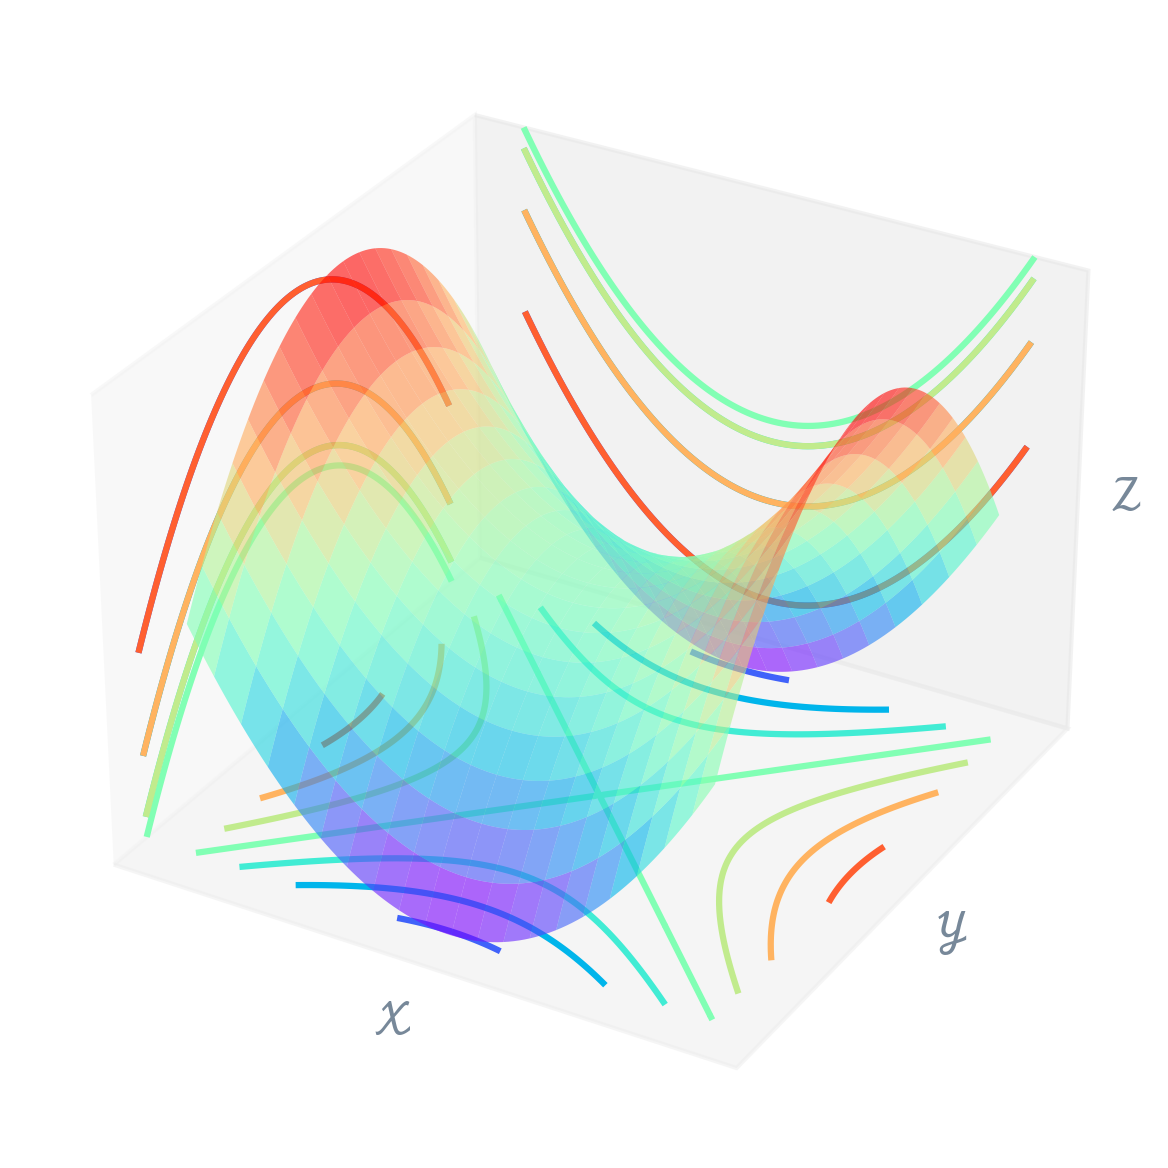
\includegraphics[width=0.9\linewidth]{./python/graph_x-pow2-sub-y-pow2_01.png}

\begin{itemize}
  \item {\bfseries $xy$平面($z=0$)} 双曲線$x^2 - y^2 =0$
  \item {\bfseries $xz$平面($y=0$)} 下に凸の放物線$z=x^2$
  \item {\bfseries $yz$平面($x=0$)} 上に凸の放物線$z=-y^2$
\end{itemize}

断面図(切り口)を順に見ていく

\br

$xz$平面における断面は、$y=0$を代入すればわかる

すると$z=f(x,0)=x^2$で、$xz$平面において下に凸の放物線になる

\br

今度は$x$を止めて、$y$を動かす

$xyz$空間の中で、$x=\text{定数}$は$yz$平面に平行な平面となる

たとえば$x=0,1,2,\cdots$とすると、順に$z=-y^2, z=1-y^2, z=4-y^2,\cdots$となり、いずれも上に凸の放物線になる

\br

下に凸の放物線(吊り下げたひも)の各点に、上に凸の放物線(針金)を順に貼り付けていくと、$z=x^2-y^2$のグラフが得られる

\sectionline

曲面$z=x^2-y^2$の局所的な形状は、身近なところにもあちこちに現れている

\br

日本の数学用語では、このグラフの原点を、山の峠にちなんで\keyword{峠点}とよぶ

西洋では、乗馬にちなんで\keyword{鞍点}とよぶ

乗馬するとき、馬の背の凹んでいるところに鞍を置いてまたがるが、その形状は峠とそっくり

\br

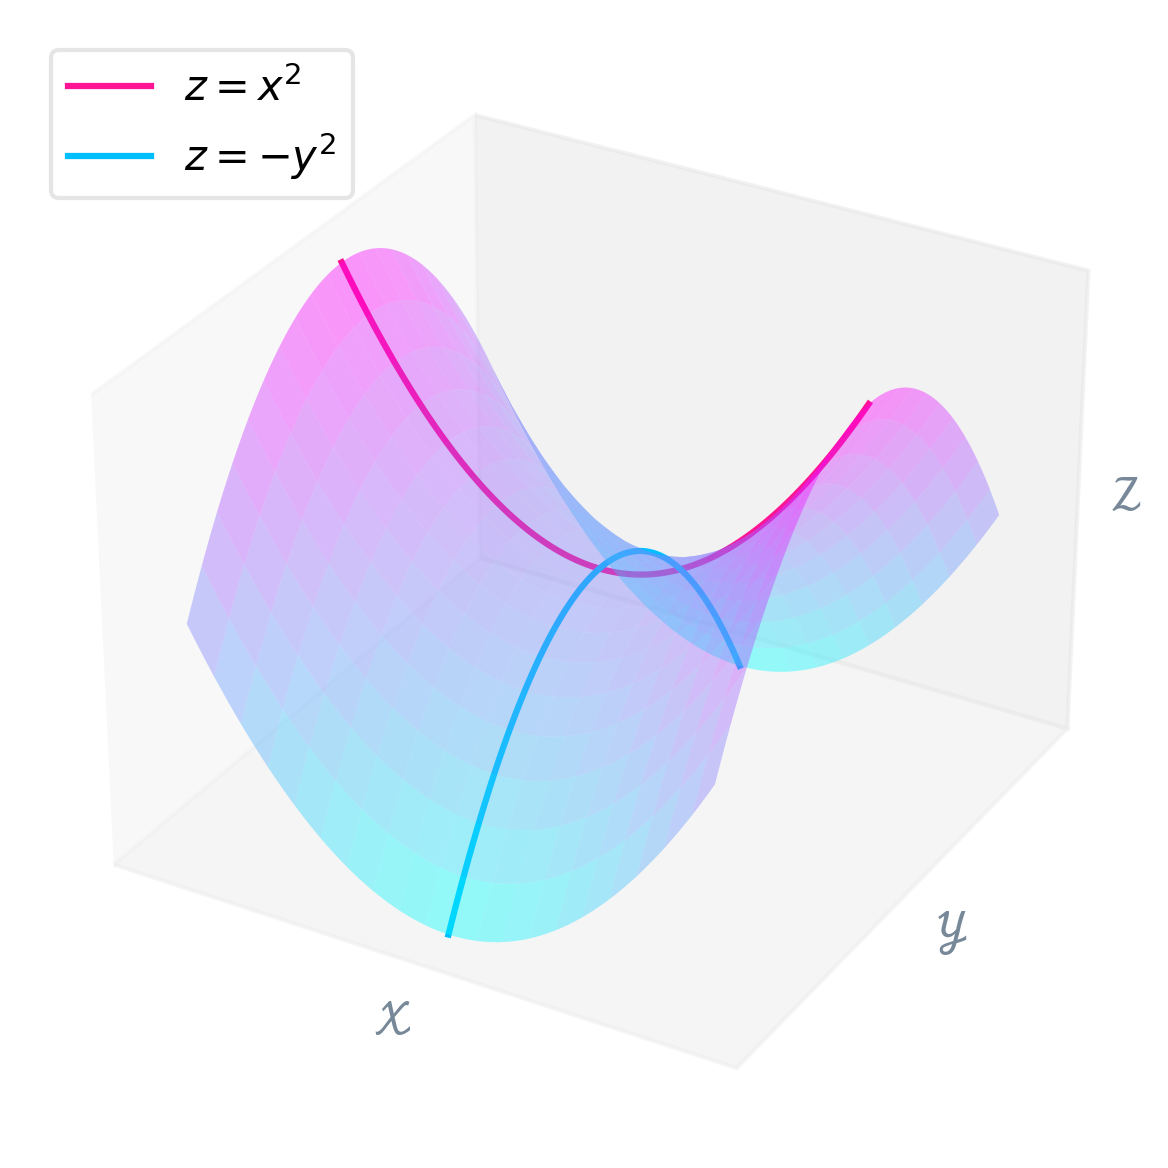
\includegraphics[width=0.9\linewidth]{./python/graph_x-pow2-sub-y-pow2_02.png}

山が連なっているような山脈を越えて向こう側に行きたいとすると、できるだけ登りが少ない経路を選ぶだろう

このような往来によって踏み固められてできた道が「山脈越えの道」(グラフでは$x=0$の場合の放物線$z = -y^2$)

\br

旅人が山脈越えの道を登っていくと、峠はその道沿いではいちばん高い地点になっている

峠で左右を見ると、山が続いている($x=\text{定数}$の場合の放物線)

\br

いま登ってきた山脈越えの道と垂直に交わっている尾根道があるかもしれない(グラフでは$y=0$の場合の放物線$z = x^2$)

尾根道沿いに歩けば、峠はその前後ではいちばん低い場所になっている

\br

これは特定の峠の話ではなく、峠の形状の普遍的な性質を示している

\section{等高線を用いて2変数関数を見る}

等高線は、2変数関数の増減を手軽に紙の上で可視化する方法

\br

2変数の関数$f(x, y)$が与えられたとき、
\begin{equation*}
  f(x, y) = \text{定数}
\end{equation*}
となるような点$(x, y)$を集めて得られる曲線を\keyword{等高線}という

\sectionline

2次元空間を可視化する方法をまとめると、

\begin{description}
  \item[グラフ(曲面)を立体模型で表す]
  \item[グラフを鳥瞰図として平面に書く] 3次元空間の中で視点を1つ選んで、$z=f(x,y)$の曲面を「風景」として平面に描く
  \item[$f(x,y)$の大きさに応じて濃淡をつける] 2次元の図で濃淡という「次元」を加えて2変数関数を見る
  \item[$f(x,y)=\text{一定}$の曲線(等高線)を描く] 2次元の図で2変数関数を表す(次元を増やす必要がない)
\end{description}

\section{ボールが転がる方向}

$x$を東西方向の位置、$y$を南北方向の位置、$f(x,y)$を点$(x,y)$における標高とし、$z=f(x,y)$のグラフが野山の形状を表しているとすると、偏微分$f_x$や$f_y$は、次のような意味を持っている

\sectionline

\paragraph{例}

$f(x,y)$が東西方向の位置$x$、南北方向の位置$y$の地点の標高を表す場合、偏微分$f_x$は、東西方向の勾配、$f_y$は南北方向の勾配である

\sectionline

実はこの2つの量$f_x, \, f_y$は東西や南北の方向だけではなく、この地点における全方位、たとえば北東の方向に進むときも傾斜の情報も持っている

\br

たとえば、野山になだらかな斜面があったとすると、斜面は空間の中の曲面と考えることができる

ここで、次のような問題を考えてみる

\br

\paragraph{問題}
東に1m進むと5cm高くなっており、北に1m進むと10cm低くなっている斜面にボールを置くと、どの方向に転がり出すか?また、この斜面で高さが一定になる方向はどの向きか?

\br

もしこの野山に雪が積もっていてスキーをするとすれば、
\begin{itemize}
  \item 直滑降では、最大傾斜の方向(ボールが転がり出す方向)を意識する
  \item 斜面を登るときは、高さが一定の方向にスキー板を向けて滑らないように横歩きする
\end{itemize}

高さが一定になる方向は、最大傾斜の方向(ボールが転がり出す方向)と垂直になっているはず(そうでなければ、スキー板が滑って降下が始まってしまう)

\br

ボールが転がり出す方向は、
\begin{itemize}
  \item 「東の方が高い」という情報だけを見ると、西の方に転がるだろう
  \item 「北の方が低い」という情報だけを見ると、北の方に転がるだろう
\end{itemize}
両方合わせると、だいたい北西の方向に転がるはず

さらに、東西よりは南北の方が勾配がきついので、北西方向よりやや北寄りに転がると推測できる

\sectionline

この推測では、「東西方向の勾配と南北方向の勾配」というデータだけで「ボールの転がり出す方向が決まりそうだ」という直観が土台になっている

\br

全方位に対する勾配の情報を集めなくても、たった2つの方向(たとえば東西と南北)の勾配の情報があれば、斜面の傾きが決定される

\sectionline

\subparagraph{接平面}

自分が立っている地点で、その斜面に接するように大きな板を置くことを想像してみる

その板は、東に1m進むと5cm高くなり、北に1m進むと10cm低くなるはず

\br

ボールをこの斜面に置いて転がり出す方向は、この板の上にボールを置いて転がり出す方向と一致すると考えられる

同様に、この地点で高度が一定になる方向(スキー板が滑らない方向)は、この板の上で考えても同じはず

\br

もちろん、現在地点が変われば斜面の傾斜も変わる

この問題を別の地点で解く場合は、その地点に合わせた別の板を使えばよい

\br

それぞれの地点で斜面に接する「大きな板」は、\keyword{接平面}という概念を表している

\sectionline

\subparagraph{接平面の方程式の決定}

接平面を数式で表すために、現在地を原点にし、$x$を東西方向の座標、$y$を南北方向の座標、$z$を上下方向の座標とする

そうすると、この地点$(0,0,0)$における接平面は、適当な実数$a,\, b$を用いて、
\begin{equation*}
  z = ax + by
\end{equation*}
と表される

\br

出発点から東西方向に動くというのは、$y=0$を固定して$x$だけを動かすことを意味する

したがって、この大きな板の上(接平面上)でこの点の高度は$z=ax$となるので、東西方向の勾配データから、
\begin{equation*}
  a = \dfrac{5}{100}
\end{equation*}

\br

同じように南北方向に動く場合を考えると、$z=by$の係数$b$は南北方向の勾配なので、
\begin{equation*}
  b = -\dfrac{10}{100}
\end{equation*}

\br

このようにして、東西方向の勾配と南北方向の勾配という2つのデータだけで、接平面の方程式が
\begin{equation*}
  z = \dfrac{5}{100}x - \dfrac{10}{100}y
\end{equation*}
と決定された

\sectionline

\paragraph{考え方の筋道}

\begin{enumerate}
  \item 曲面を平面(この地点における接平面)に置き換える
  \item 接平面に対して問題を解く
\end{enumerate}

\sectionline

問題によって何を求めたいかは異なるが、ステップ1で問題を扱いやすい形に近似し、ステップ2で扱いやすくなった問題を解くというアプローチ

\br

\subparagraph{ステップ1}\quad

より簡単な扱いやすい図形や数式で近似しようというのが基本方針

ここで局所的な近似を見つける際に、\keyword{偏微分}が活躍する

\br

\keyword{曲がったものを局所的にまっすぐなもので近似する}という考え方は、いろいろな場面で利用されている

たとえば、地域の地図を作成する場合、地球が丸いことは無視して、あたかも地球が平らであるかのように描く

丸い地球を平面で近似しても、狭い地域ならば誤差はわずかである

\br

\subparagraph{ステップ2}\quad

ステップ2では、直線や平面といった「まっすぐな」図形を扱う

直線(接線)や平面(接平面)を表す方程式は1次式で表されるため、ステップ2は1次式の問題になる

\br

直線・平面という1, 2次元の図形や、変数が2,3個の連立1次方程式なら簡単だが、次元が高かったり、変数が多くなったりすると、直観ではつかみにくくなる

このような高次元のことを系統的に扱うのが\keyword{線形代数}である

\end{document}
